
\documentclass{article}

\usepackage{palatino}
\usepackage{euler}
\usepackage{graphicx}

\begin{document}
\section{Non-bonded contacts}


From Wikipedia, the Lennard-Jones energy $V_{\mathit{ji}}(r)$ is

\begin{equation}
  \label{eq:1}
  V_{\mathit{lj}}(r) = 4 \epsilon \left[ \frac{\sigma}{r}^{\mathit{12}} - \frac{\sigma}{r}^{6} \right]
\end{equation}

Where

\begin{trivlist}
\item $r$ is the distance between the pair of atoms and
\item $\sigma$ is where the function crosses the $x$-axis.
\end{trivlist}

When using distances from the dictionary though, I am determining $r_{\mathit{min}}$ rather than $\sigma$.
$r_{\mathit{min}}$ is the optimal value (energy minimum) for the atom pair (\emph{e.g.} 2.8 \AA\ for an H-bond).

We know that

\begin{equation}
  \label{eq:2}
  r_{\mathit{min}} = 2^{\frac{1}{6}} \sigma
\end{equation}

so substituting that, we get 

\begin{equation}
  \label{eq:3}
  V_{\mathit{lj}}(r) = \epsilon \left[ \frac{r_{\mathit{min}}}{r}^{\mathit{12}} - 2 \frac{r_{\mathit{min}}}{r}^{6} \right]
\end{equation}

Now if we say:

\begin{equation}
  \label{eq:4}
  \alpha = \frac{r_{\mathit{min}}}{r}
\end{equation}

we get

\begin{equation}
  \label{eq:3}
  V_{\mathit{lj}}(r) = \epsilon \left[ \alpha^{\mathit{12}} - 2 \alpha^{6} \right]
\end{equation}

and that is the form that I use in \emph{Coot}.

The derivative of $V_{\mathit{lj}}(r)$ is

\begin{equation}
  \label{eq:derivative}
  \frac{\partial V_{\mathit{lj}}(r)}{\partial r} = \frac{\partial V_{\mathit{lj}}}{\partial \alpha} . \frac{\partial \alpha}{\partial r}
\end{equation}

\emph{i.e.}

\begin{equation}
  \label{eq:derivative}
  \frac{\partial V_{\mathit{lj}}(r)}{\partial r} = 12 \epsilon \left[ \alpha^{\mathit{11}} - \alpha^{5} \right] . \left( \frac{-r_{\mathit{min}}}{r^2} \right)
\end{equation}


\begin{figure}
  \centering
  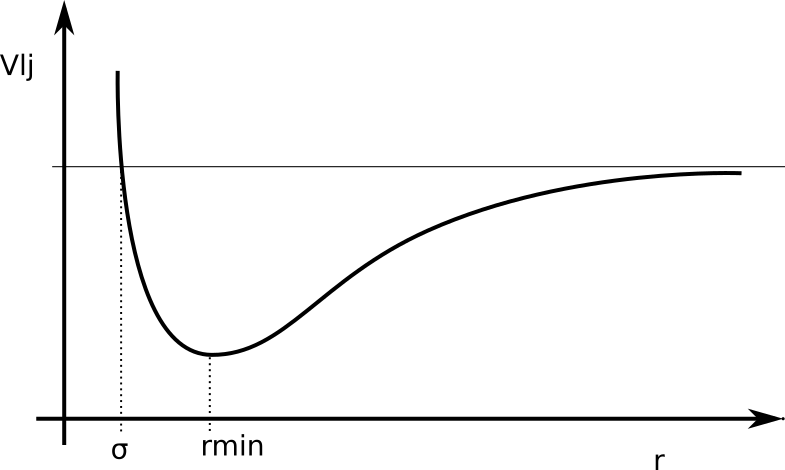
\includegraphics[width=8cm]{lennard-jones.png}
  \caption{Lennard-Jones.  $r_{\mathit{min}} = 2^{\frac{1}{6}} \sigma$}
  \label{fig:lennard-jones}
\end{figure}

\end{document}
